\subsection{Model Selection and Definition}
Despite being grounded in IoT and proximity sensing, our system still operates under partial observability. Each agent (driver) must make decisions without access to a global view of the environment. This challenge demands efficient coordination mechanisms. Research shows that Graph Neural Network (GNN)-based communication and centralized critic methods significantly improve agent performance in cooperative MARL (Multi-Agent Reinforcement Learning) environments like traffic or parking optimization\footcite{article}.

These findings highlight the need for communication mechanisms in our implementation—whether for shared observations, intent signalling, or updates about false positives/negatives. Such mechanisms become essential for agents to reconcile partial, noisy observations into actionable collective knowledge.

Our architecture is based on the Soft Actor-Critic (SAC) algorithm within a Centralized Training with Decentralized Execution (CTDE) framework. The central critic has access to global mesh data during training, while each actor acts independently at inference time using local sensor and Bluetooth inputs. This hybrid approach provides both training robustness and deployment flexibility.

The actor network is modeled as a Multi-Layer Perceptron (MLP) with two hidden layers of 256 neurons each, using LeakyReLU activations and a Softmax output. This structure balances expressivity with computational simplicity. For the critic, we explore three options:
\begin{itemize}
    \item \textbf{MLP:} Efficient for small input sizes; fast and easy to implement.
    \item \textbf{GNN:} Scales across fleet sizes; enables message passing between nodes.
    \item \textbf{Graph + Attention Pooling (G+A):} Learns contextual factors like time-of-day or regional bias through attention mechanisms.
\end{itemize}
To improve generalization, we incorporate regularization techniques such as L1/L2 penalties and dropout.

\begin{figure}[H]
    \centering
    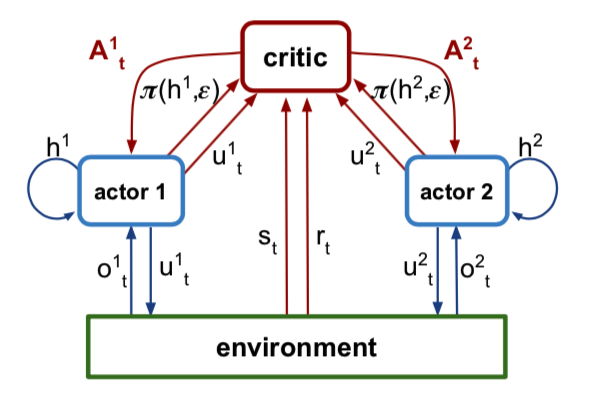
\includegraphics[width=0.8\linewidth]{Figures/c_critic.png}
    \captionsetup{justification=centering}
    \caption{Centralized critic architecture under CTDE.\footcite{Whiteson2020FactoredValue}}
    \label{fig:central-critic}
\end{figure}
\footnotetext[9]{Adapted from \cite{Whiteson2020FactoredValue}.}

To benchmark alternative MARL methods, we conducted a literature survey and compared several state-of-the-art algorithms\footcite{amato2024introductioncentralizedtrainingdecentralized} in terms of credit assignment, scalability, and applicability to a city-scale parking mesh\footcite{article}. The results are summarized below.

\begin{table}[htp]
\centering
\caption{COMA (Counterfactual MA-AC)}
\small
\begin{tabularx}{\linewidth}{>{\bfseries}p{3.5cm} >{\RaggedRight\arraybackslash}X}
\toprule
Credit Assignment & Per-agent counterfactual baseline \\
Strengths & Low-variance gradients on \textit{small} teams \\
Weaknesses & Critic input grows with $N$; unworkable when thousands of agents share a road graph \\
\bottomrule
\end{tabularx}
\end{table}

\FloatBarrier

\begin{table}[htp]
\centering
\caption{QMIX / VDN}
\small
\begin{tabularx}{\linewidth}{>{\bfseries}p{3.5cm} >{\RaggedRight\arraybackslash}X}
\toprule
Credit Assignment & Monotonic mixing of per-agent Q-values \\
Strengths & Scales to hundreds of agents \\
Weaknesses & Monotonic constraint fails under non-linear interactions (e.g., two cars blocking one lane) \\
\bottomrule
\end{tabularx}
\end{table}

\FloatBarrier

\begin{table}[htp]
\centering
\caption{MADDPG / MA-SAC}
\small
\begin{tabularx}{\linewidth}{>{\bfseries}p{3.5cm} >{\RaggedRight\arraybackslash}X}
\toprule
Credit Assignment & Central critic over joint observations \\
Strengths & Handles continuous control; replay-buffer friendly \\
Weaknesses & Critic overfits when $N > 50$; loses locality information \\
\bottomrule
\end{tabularx}
\end{table}

\FloatBarrier

\begin{table}[H]
\centering
\caption{MAGAC (Multi-Agent Graph Soft Actor Critic)}
\small
\begin{tabularx}{\linewidth}{>{\bfseries}p{3.5cm} >{\RaggedRight\arraybackslash}X}
\toprule
Credit Assignment & GNN critic with “soft” counterfactuals \\
Strengths & Near-linear scaling; exploits road topology; variable team sizes \\
Weaknesses & Requires neighbor graph and message-passing layers \\
\bottomrule
\end{tabularx}
\end{table}


Based on the above analysis, while COMA and QMIX have proven value in constrained team settings, they fail to scale to large agent populations or complex topologies. MAGAC emerges as the most promising candidate for our scenario, combining scalability, robustness, and architectural alignment with our graph-based parking mesh.

\subsubsection*{Soft Actor-Critic GNN Component}

Graph Neural Networks (GNNs) generalize convolution to problems whose natural structure is a graph—a set of nodes (vehicles) linked by edges (Bluetooth connections). Instead of sliding a fixed-size kernel across pixels, a GNN lets every node exchange “messages” with its neighbors, aggregate what it hears, and update its own hidden state. By stacking multiple message-passing layers, information propagates hop-by-hop—enabling each vehicle to reason not only about the parking bays it sees but also about availability cues relayed from cars two or three streets away.

At each message-passing step, every sender node \( j \) transforms its current embedding \( h_j^{(\ell - 1)} \) using a learned weight matrix \( W \) (or a small MLP). This transformed vector is concatenated with the receiver’s embedding \( h_i^{(\ell - 1)} \), and the pair is passed through an activation function such as \(\text{LeakyReLU}\) to produce a raw compatibility score \( e_{ij} \):

\[
e_{ij} = \text{LeakyReLU}(W[h_i^{(\ell - 1)} \Vert h_j^{(\ell - 1)}])
\]

The scores \( e_{ij} \) for all neighbors of node \( i \) are normalized using a softmax to yield attention coefficients \( \alpha_{ij} \):

\[
\alpha_{ij} = \frac{\exp(e_{ij})}{\sum_{k \in \mathcal{N}(i)} \exp(e_{ik})}
\]

These coefficients act as an adaptive attention kernel: for instance, a car that recently confirmed a vacancy may receive a high weight, while a distant or outdated neighbor receives little influence.

The reason GNNs are well-suited to our Parking Mesh system is scalability. The same shared weight matrix \( W \) operates whether there are 50 or 50{,}000 cars in the graph. Unlike an MLP critic that flattens the environment into a fixed-size vector, a GNN respects the road network’s structure, focusing computation on meaningful local interactions. This results in \textbf{linear scalability} with the number of edges—an essential feature for a real-time urban system.

\subsubsection*{Target-Network Implementation}

To mitigate the moving-target problem in off-policy learning, we maintain a separate \textbf{target critic network}—a periodically updated copy of the main GNN-based critic—that provides stable Q-value estimates during training. After each critic update, we softly update the target network parameters using \textbf{Polyak averaging}:

\[
\theta_{\text{target}} \leftarrow (1 - \tau)\,\theta_{\text{target}} + \tau\,\theta_{\text{critic}}
\]

where \( \tau = 0.005 \) is the update rate.

Rather than applying this update at every gradient step, we accumulate critic gradients over three mini-batches before performing both the optimizer step and the Polyak update. This staggered update reduces jitter in the target values and improves training stability.

The target network is initialized as an exact copy of the main critic at the start of training and then gradually tracks it through these soft updates. When computing Bellman backups during training, we use \textbf{clipped double Q-learning}—taking the minimum of the two target critic heads—to reduce overestimation bias:

\[
Q_{\text{target}} = \min\big(Q_{\text{target}}^{(1)},\, Q_{\text{target}}^{(2)}\big)
\]

This clipped estimate helps ensure that our centralized critic provides a \textbf{stable and conservative learning signal} for the decentralized actor policies, which is crucial for convergence in multi-agent systems like Parking Mesh.

​
